\section{Metrics}
Since our dataset is unpaired, pixel-based metrics are not fit for performance evaluation. 
This implies that only statistically based metrics are viable.
One such metric is the Fréchet Inception Distance (FID) \cite{DBLP:journals/corr/HeuselRUNKH17}, widely used for evaluating the quality of generated images and specifically GANs.
Typically, a lower FID score indicates greater fidelity of the generated images to the real target modality.
We note here that while the density and coverage (DC) \cite{naeem2020reliable} metric is the most recent and popular approach for evaluating GANs, its coverage component is irrelevant for I2I tasks because the output's content is necessarily conditioned on the input.
Therefore, DC has no added value over FID in our case, and we use FID as our sole numerical evaluation metric.

\section{Experimental setup}
As a rule of thumb, the FID metric requires test sets of about $10,000$ images from each modality to be indicative of their true statistical distribution. 
This clearly limits the amount of data left for training and validation.
Thus, only $1000$ images were used for training and $100$ for validation per modality, resulting in a total of $2200$ images.

To fairly assess the method's contribution, we first trained our baseline models (CycleGAN, CUT) and fine-tuned their original hyperparameters and design choices.
Consequently, the following changes were implemented to achieve optimal FID score on our dataset: 
\begin{itemize}
    \item Generator's bottleneck was implemented using 6 residual blocks (instead of 9).
    \item Learning-rate was set to $5 \times 10^{-4}$ (instead of $2 \times 10^{-4}$).
    \item A 2-Batch size was used (instead of 1)
    \item The total number of epochs was 100 (instead of 200)
\end{itemize}

The same set of hyperparameters and design choices were applied as is for training our proposed methods and their ablative configurations.
For each model configuration, FID was calculated at the end of every epoch.
The minimum (best) FID score over all epochs was treated as the score of that configuration.
We note that since the FID is an evaluation metric, it should in essence be run only at test time, after training has already ended. 
Nevertheless, as the hyperparameters were fixed for all configurations, there was no flaw in calculating it at the end of every epoch, because it is calculated based on an orthogonal set of samples, which is the test set in our case.

\section{Results}
\subsection{Quantitative}
Typically, numerical scores are obtained by training a network and evaluating it once.
However, as the loss function is highly non-convex \wrt the network's parameters, the local minimum to which the network converges is highly dependent on its weight initialization.
The findings of \cite{picard2021torch} further illustrate that a network trained once (\ie, with a single weight initialization) can have an outlier score that is much better or much worse than the average.

Therefore, we chose a statistical approach to evaluate and compare the different configurations.
For each configuration, we trained and evaluated the FID score 10 consecutive times, where we randomly initialized the weights in every training-evaluation cycle.
We then calculated the mean and standard deviation of the 10 FID scores and used them as criteria for comparison with the other configurations.
This approach reduces the sensitivity to the randomness of the weight initialization, and provides a measure for the training procedure's consistency, which can be inferred from the standard deviation.

The numerical comparison between the different configurations can be found in Table \ref{tbl:results}.
We tested every possible configuration of our propositions, \ie, with and without providing the intrinsic temperatures  to the deep generator, and with and without fusing the deep generator with the physical estimator.
All configurations were tested on top of both baseline models (CycleGAN and CUT).

\begin{table}
    \centering
    \begin{tabular}{| c  c  c  c || c  c |}
        % \toprule
        \multicolumn{4}{c}{Configuration} & \multicolumn{2}{c}{FID} \\
        % \hline\hline
        \hline
        % \midrule
        Backbone & Int & Phys & Caption & Mean & Std\\
        \hline
        \multirow{4}{4em}{\centering CycleGan}  & \xmark & \xmark & Baseline    & 51.05             & 9.82\\      
                                                & \xmark & \cmark &             & 35.54             & 3.72\\ 
                                                & \cmark & \xmark &             & 50.17             & 8.89\\
                                                & \cmark & \cmark & PETIT       & \textbf{33.8}     & \textbf{1.23}\\
        \hline
        \multirow{4}{4em}{\centering CUT}       & \xmark & \xmark & Baseline    & 38.43             & 1.52\\
                                                & \xmark & \cmark &             & 29.85             & \textbf{0.99}\\
                                                & \cmark & \xmark &             & 48.88             & 1.46\\
                                                & \cmark & \cmark & PETIT       & \textbf{27.35}    & 1.01\\
        \hline
        % \bottomrule
    \end{tabular}
    \caption{Comparison of FID score statistics between the different configurations (the lower the better). \emph{Int} stands for intrinsic temperature and \emph{Phys} for physical estimator.}
    \label{tbl:results}
\end{table}

PETIT was found to dominate all other configurations with both backbones.
Specifically, compared to the baseline configurations, PETIT achieved an approximately $50\%$ mean FID improvement and a significantly improved standard deviation, indicating a more consistent training procedure.
Another interesting observation was that all configurations involving the physical estimator outperformed their counterparts by a large margin, in terms of both mean and standard deviation.
On the other hand, the intrinsic temperature information alone did not seem to have a significant impact on the results, and was only helpful when combined with the physical estimator.
This suggests that the physically estimated prior information steers the model toward points on the manifold where the intrinsic temperature information is locally beneficial.

\subsection{Qualitative}
In accordance with the quantitative results, the monochromatic outputs produced by PETIT seem to be of superior quality compared to all other configurations.
Generally speaking, PETIT's outputs incur less spurious artifacts and exhibit stronger fidelity to real monochromatic modality. 
An impression of the discussed superiority can be obtained from the examples in Figure \ref{fig:qual_comp}.
Due to space limitations, we only display the results of the CUT backbone-based baseline and PETIT configurations.
Real unpaired monochromatic images are also displayed in juxtaposition to the generated outputs for an impression of the modality's true nature.

\begin{figure}[H]
    % 1st Row
    \centering
    \begin{subfigure}[b]{0.24\textwidth}
        \centering
        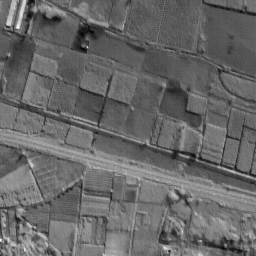
\includegraphics[width=\textwidth]{../figs/outputs/pan/71.png}
    \end{subfigure}
    \hfill
    \begin{subfigure}[b]{0.24\textwidth}
        \centering
        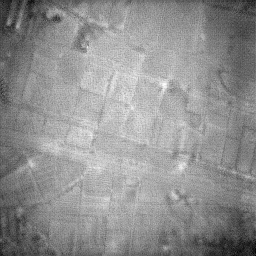
\includegraphics[width=\textwidth]{../figs/outputs/cut/71.png}
    \end{subfigure}
    \hfill
    \begin{subfigure}[b]{0.24\textwidth}
        \centering
        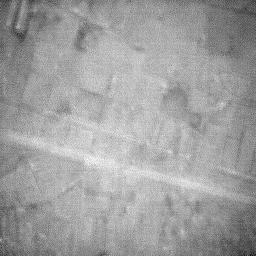
\includegraphics[width=\textwidth]{../figs/outputs/petit/71.png}
    \end{subfigure}
    \hfill
    \begin{subfigure}[b]{0.24\textwidth}
        \centering
        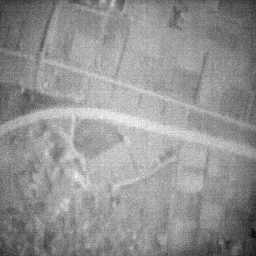
\includegraphics[width=\textwidth]{../figs/outputs/mono/605.png}
    \end{subfigure}      
    
    % 2nd Row
    \centering
    \begin{subfigure}[b]{0.24\textwidth}
        \centering
        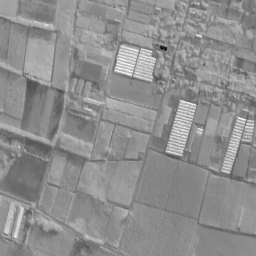
\includegraphics[width=\textwidth]{../figs/outputs/pan/24.png}
    \end{subfigure}
    \hfill
    \begin{subfigure}[b]{0.24\textwidth}
        \centering
        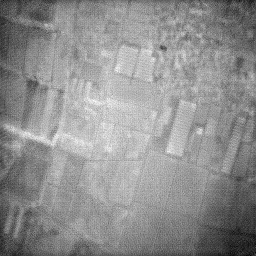
\includegraphics[width=\textwidth]{../figs/outputs/cut/24.png}
    \end{subfigure}
    \hfill
    \begin{subfigure}[b]{0.24\textwidth}
        \centering
        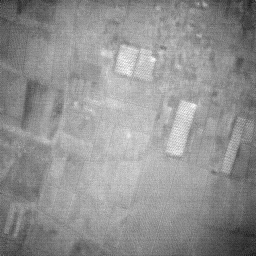
\includegraphics[width=\textwidth]{../figs/outputs/petit/24.png}
    \end{subfigure}
    \hfill
    \begin{subfigure}[b]{0.24\textwidth}
        \centering
        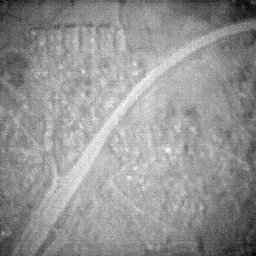
\includegraphics[width=\textwidth]{../figs/outputs/mono/508.png}
    \end{subfigure}    
    
    % 3rd Row
    \begin{subfigure}[b]{0.24\textwidth}
        \centering
        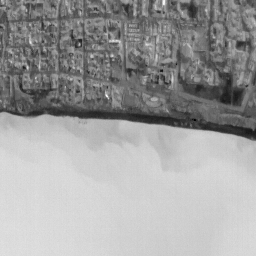
\includegraphics[width=\textwidth]{../figs/outputs/pan/28.png}
        \subcaption{Pan (input)}
        \label{fig:pan}
    \end{subfigure}
    \hfill
    \begin{subfigure}[b]{0.24\textwidth}
        \centering
        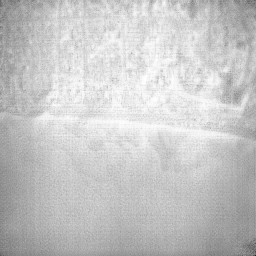
\includegraphics[width=\textwidth]{../figs/outputs/cut/28.png}
        \subcaption{CUT (baseline)}
        \label{fig:cut}
    \end{subfigure}
    \hfill
    \begin{subfigure}[b]{0.24\textwidth}
        \centering
        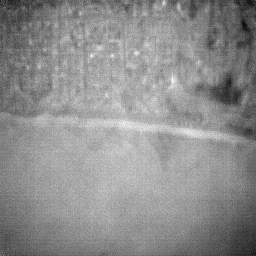
\includegraphics[width=\textwidth]{../figs/outputs/petit/28.png}
        \subcaption{PETIT (ours)}
        \label{fig:petit}
    \end{subfigure}
    \hfill
    \begin{subfigure}[b]{0.24\textwidth}
        \centering
        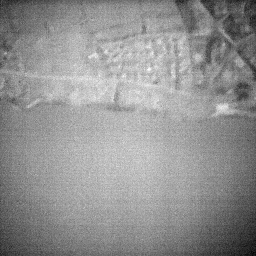
\includegraphics[width=\textwidth]{../figs/outputs/mono/994.png}
        \subcaption{Mono (ref)}
        \label{fig:mono}
    \end{subfigure}

    \caption{Qualitative comparison. (a) Panchromatic (Pan) input. (b) Baseline output. (c) PETIT output. (d) Real unpaired monochromatic image (Mono) for reference.}
    \label{fig:qual_comp}
\end{figure}